\documentclass{beamer}
\beamertemplatenavigationsymbolsempty
\usecolortheme{beaver}
\setbeamertemplate{blocks}[rounded=true, shadow=true]
\setbeamertemplate{footline}[page number]
%
\usepackage[utf8]{inputenc}
\usepackage[english,russian]{babel}
\usepackage{amssymb,amsfonts,amsmath,mathtext}
\usepackage{subfig}
\usepackage[all]{xy} % xy package for diagrams
\usepackage{array}
\usepackage{multicol}% many columns in slide
\usepackage{hyperref}% urls
\usepackage{hhline}%tables
\usepackage{algorithm}
\usepackage{algpseudocode}
% Your figures are here:
\graphicspath{ {fig/} {../figures/} }

%----------------------------------------------------------------------------------------------------------
\title[\hbox to 56mm{Ускоренные безградиентные методы}]{Ускоренные методы нулевого порядка в гладкой выпуклой стохастической оптимизации}
\author[Ф.\,А. Хафизов]{Фанис Адикович Хафизов}
\institute{Московский физико-технический институт}
\date{\footnotesize
\par\smallskip\emph{Курс:} Автоматизация научных исследований\par (практика, В.\,В.~Стрижов)/Группа 105
\par\smallskip\emph{Эксперт:} к.ф.-м.н А.\,Н.~Безносиков
\par\smallskip\emph{Консультант:} А.\,И.~Богданов
\par\bigskip\small 2024}
%----------------------------------------------------------------------------------------------------------
\begin{document}
%----------------------------------------------------------------------------------------------------------
\begin{frame}
\thispagestyle{empty}
\maketitle
\end{frame}
%-----------------------------------------------------------------------------------------------------
\begin{frame}{Цель исследования}
\begin{block}{Цель:}
\begin{itemize}
 \item Создать ускоренный безградиентный метод решения задачи безусловной гладкой стохастической оптимизации
 \item Доказать сходимость в случае детерминированного шума
 \item Поставить численный эксперимент и сравнить с методом Нестерова и градиентным спуском в случаях детерминированного и стохастического шума
\end{itemize}

\end{block}
\end{frame}
%-----------------------------------------------------------------------------------------------------
\begin{frame}{Доклад с одним слайдом}

\begin{columns}[c]
    \column{0.5\textwidth}
    $$\min\limits_{x \in \mathbb{R}^d} f(x)$$
    \column{0.5\textwidth}
    $$f_\delta (x) = f(x) + \delta (x).$$
\end{columns}

$$\widetilde{\nabla}_i f_\delta (x) := \frac{f_\delta (x + \tau e_i) - f_\delta (x - \tau e_i)}{2\tau} e_i$$

\begin{columns}[c]
    \column{0.5\textwidth}
    \begin{figure}
    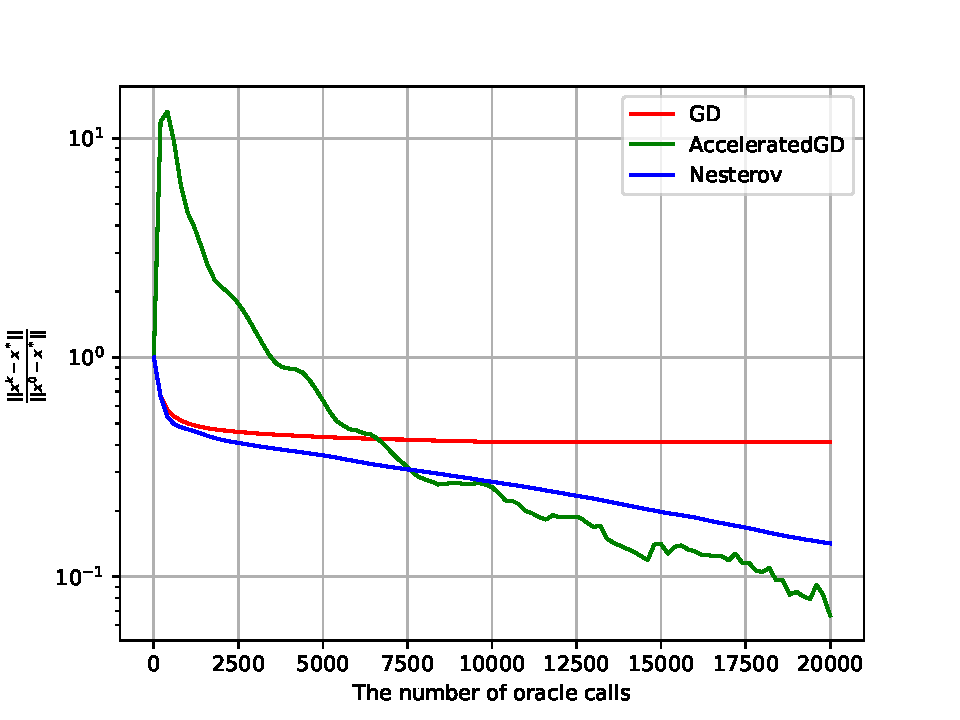
\includegraphics[width=1.0\textwidth]{Deterministic_quadratic_GD_AGD_Nesterov_15.pdf}
        \caption*{Зависимость $\frac{\|x^k - x^*\|}{\|x^0 - x^*\|}$ от числа итераций, квадратичная задача минимизации}
    \end{figure}

    \column{0.5\textwidth}
    \begin{figure}
    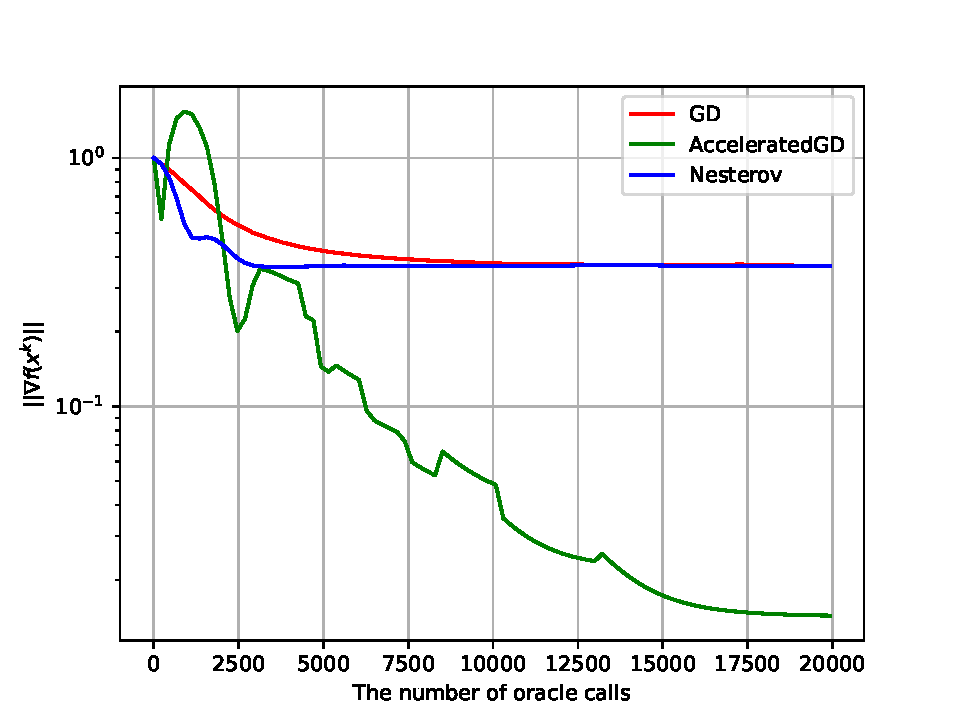
\includegraphics[width=1.0\textwidth]{Non_stochastic_Logreg_GD_AGD_Nesterov_15_1e-07_1e-05.pdf}
        \caption*{Зависимость $\|\nabla f(x^k)\|$ от числа итераций, задача логистической регрессии}
    \end{figure}
\end{columns}

\end{frame}

%-----------------------------------

\begin{frame}{Литература}

\begin{itemize}
 \item Aleksandr Beznosikov, Sergey Samsonov, Marina Sheshukova, Alexander Gasnikov, Alexey Naumov, Eric Moulines. First Order Methods with Markovian Noise: from Acceleration to Variational Inequalities. 2023.
 \item Andrey Veprikov, Alexander Bogdanov, Vladislav Minashkin, Aleksandr Beznosikov, Alexander Gasnikov. New Aspects of Black Box Conditional Gradient: Variance Reduction and One Point Feedback. 2024.
 \item Eduard Gorbunov, Pavel Dvurechensky, Alexander Gasnikov. An Accelerated Method for Derivative-Free Smooth Stochastic Convex Optimization. 2020.
\end{itemize}

\end{frame}

%-----------------------------------

\begin{frame}{Постановка задачи. Детерминированный случай}
\begin{block}{Дано}
 $f: \mathbb{R}^d \to \mathbb{R}$ --- $\mu$-сильно выпуклая, $L$-гладкая функция. Доступ к оракулу нулевого порядка $f_\delta(x) = f(x) + \delta(x)$: $|\delta(x)| \leqslant \Delta$.
\end{block}
\begin{block}{Требуется}
 Построить алгоритм, решающий задачу
 \begin{equation}
  \min\limits_{x \in \mathbb{R}^d} f(x),
  \label{determenistic_problem}
 \end{equation}

 обращаясь к оракулу $f_\delta$.
\end{block}

\end{frame}

%----------------------------------------

\begin{frame}{Постановка задачи. Стохастический случай}
\begin{block}{Дано}
 $f: \mathbb{R}^d \to \mathbb{R}$ --- $\mu$-сильно выпуклая, $L$-гладкая функция. Доступ к оракулу нулевого порядка $f_\delta(x) = f(x) + \delta(x, \xi)$: $\mathbb{E}[|\delta(x, \xi)|^2] \leqslant \Delta^2$.
\end{block}
\begin{block}{Требуется}
 Построить алгоритм, решающий задачу
 $$\min\limits_{x \in \mathbb{R}^d} f(x) := \mathbb{E}_{\xi \sim \pi}[f(x, \xi)],$$
 обращаясь к оракулу $f_\delta$.
\end{block}

\end{frame}

%--------------------------------------


\begin{frame}{Предложенный метод}

\begin{algorithm}[H]
\caption{ Accelerated Gradient Descent }
\label{agd_algorithm}
\begin{algorithmic}
\Require{stepsize $\gamma > 0$, momentums $\theta, \eta, \beta, p$, number of iterations $N$, approximation parameter $\tau > 0$.}
\State\textbf{Initialization:} choose $x^0 = x_f^0$
   \For{$k=0, 1,  \ldots, N-1$}
		\State $x_g^k = \theta x_f^k + (1 - \theta)x^k$
		\State $g^k = \sum\limits_{i = 1}^k \frac{f_\delta(x_g^k + \tau e_i) - f_\delta(x_g^k - \tau e_i)}{2\tau}e_i$
		\State $x_f^{k + 1} = x_g^k - p \gamma g^k$
		\State $x^{k + 1} = \eta x_f^{k + 1} + (p - \eta) x_f^k + (1 - p)(1 - \beta) x^k + (1 - p)\beta x_g^k$
   \EndFor
\end{algorithmic}
\end{algorithm}

\end{frame}

%-----------------------------------

\begin{frame}{Скорость сходимости}
\begin{theorem}\label{theorem1}
  Ускоренный градиентный спуск (Algorithm \ref{agd_algorithm}) имеет скорость сходимости на задаче (\ref{determenistic_problem}):
  \begin{equation}
   \begin{aligned}
   \mathbb{E}\left[\|x^N - x^*\|^2 + \frac{6}{\mu} (f(x_f^N) - f(x^*))\right] \hfill\\
   \leqslant \exp\left(- N\sqrt{\frac{p^2\mu\gamma}{3}}\right) \left(\|x^0 - x^*\|^2 + \frac{6}{\mu} (f(x_f^0) - f(x^*))\right) + \\
   + \frac{6}{\mu} \sqrt{\frac{3}{\mu L}} \left(1 + 2\sqrt{\frac{3}{\mu \gamma}}\right) d \left(\frac{L\tau}{2} + \frac{\Delta}{\tau}\right)^2,
   \label{deterministic_convergence}
   \end{aligned}
  \end{equation}
  где $\gamma \in (0, \frac{3}{4L}], \beta, \theta, \eta, p$ такие, что:

  \begin{equation}
   p \simeq (2(1 + \gamma L))^{-1}, \beta \simeq \sqrt{p^2 \mu \gamma}, \eta \simeq \sqrt{\frac{1}{\mu\gamma}}, \theta \simeq \frac{p \eta^{-1} - 1}{\beta p \eta^{-1} - 1.}
  \end{equation}

\end{theorem}
\end{frame}

\begin{frame}{Вычислительный эксперимент}
Производится сравнение с методами Нестерова и градиентного спуска. Детерминированный шум реализован округлением до 6 знака после запятой.
\begin{columns}[c]
    \column{0.5\textwidth}
    \begin{figure}
    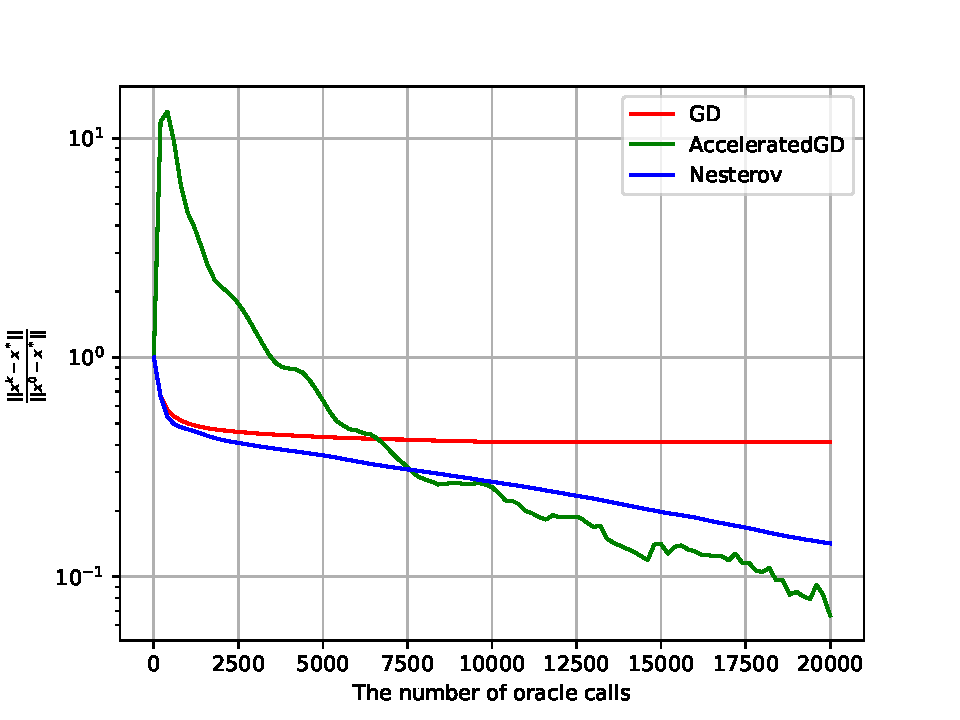
\includegraphics[width=1.0\textwidth]{Deterministic_quadratic_GD_AGD_Nesterov_15.pdf}
        \caption*{Зависимость $\frac{\|x^k - x^*\|}{\|x^0 - x^*\|}$ от числа итераций, квадратичная задача минимизации}
    \end{figure}

    \column{0.5\textwidth}
    \begin{figure}
    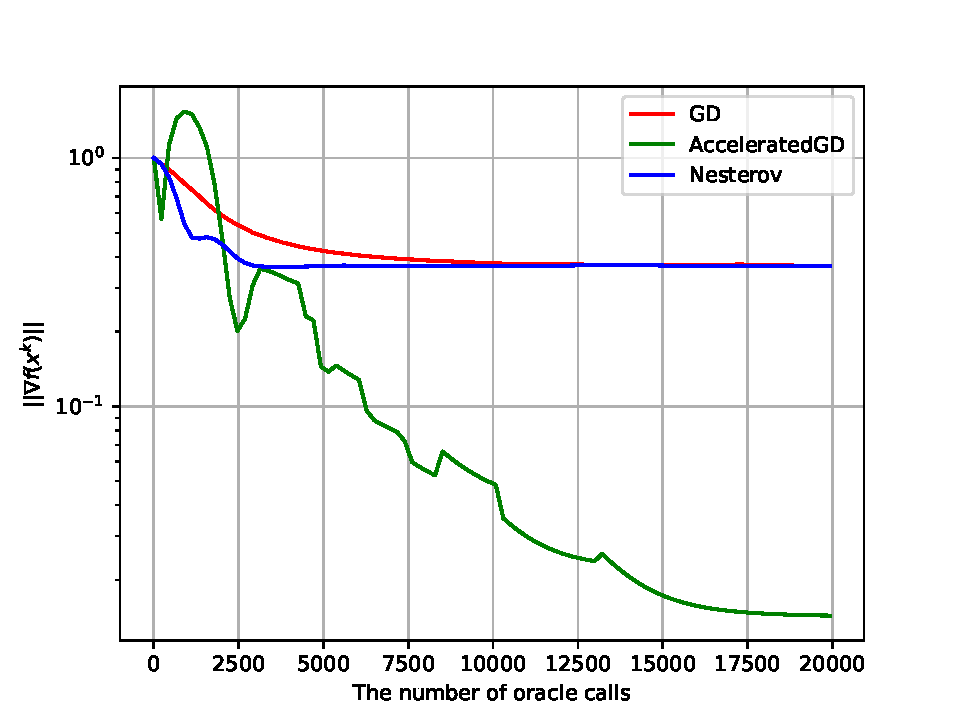
\includegraphics[width=1.0\textwidth]{Non_stochastic_Logreg_GD_AGD_Nesterov_15_1e-07_1e-05.pdf}
        \caption*{Зависимость $\|\nabla f(x^k)\|$ от числа итераций, задача логистической регрессии}
    \end{figure}
\end{columns}
\end{frame}


\begin{frame}{Анализ ошибки}
\begin{columns}[c]
    \column{0.5\textwidth}
    \begin{figure}
    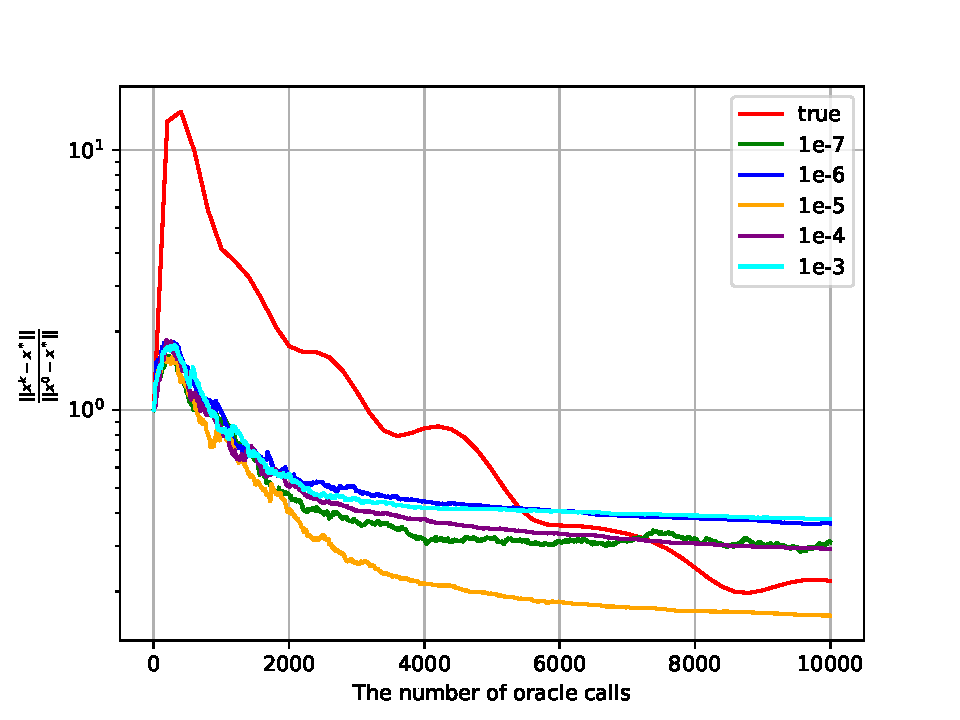
\includegraphics[width=1.0\textwidth]{Error_analysis_quadratic_sigma=1e-6.pdf}
        \caption*{Зависимость относительной ошибки $\frac{\|x^k - x^*\|}{\|x^0 - x^*\|}$ от числа оракульных вызовов для Accelerated GD с изменяющимся значением $\tau$, а также Accelerated GD с аналитически вычисленным градиентом, квадратичная задача.}
    \end{figure}

    \column{0.5\textwidth}
    \begin{figure}
    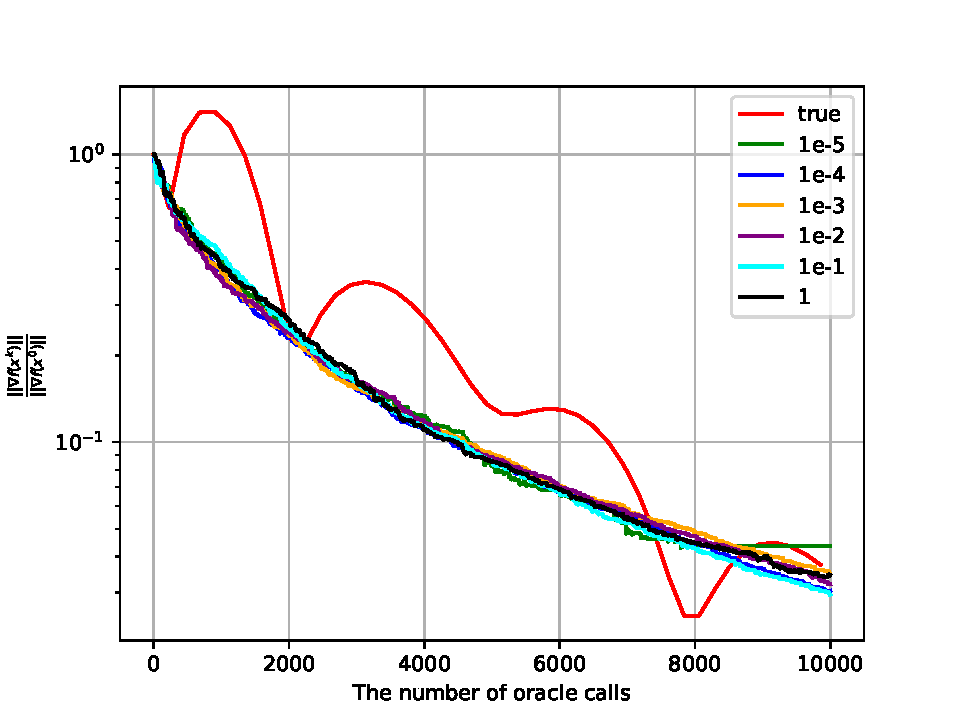
\includegraphics[width=1.0\textwidth]{Error_analysis_logreg_sigma=1e-6.pdf}
        \caption*{Зависимость относительной ошибки $\frac{\|\nabla f(x^k)\|}{\|\nabla f(x^0)\|}$ от числа оракульных вызовов для Accelerated GD с изменяющимся значением $\tau$, а также Accelerated GD с аналитически вычисленным градиентом, логистическая регрессия.}
    \end{figure}
\end{columns}
\end{frame}


\begin{frame}{Результаты}
\begin{itemize}
 \item Предложен метод нулевого порядка, решающий поставленную задачу
 \item Получена скорость сходимости на описанном классе функций
 \item Показано превосходство предложенного метода перед методом Нестерова и градиентным спуском
\end{itemize}

\begin{block}{Будущая работа}
 Развить теорию на стохастический случай.
\end{block}

\end{frame}

\end{document}
